%% REPLACE SXXXXXX with your student number
\def\studentNumber{S2827027}


%% START of YOUR ANSWERS
%% Add answers to the questions below, by replacing the text inside the brackets {} for \youranswer{ "Text to be replaced with your answer." }. 
%
% Do not delete the commands for adding figures and tables. Instead fill in the missing values with your experiment results, and replace the images with your own respective figures.
%
% You can generally delete the placeholder text, such as for example the text "Question Figure 2 - Replace the images ..." 
%
% There are 6 TEXT QUESTIONS. Replace the text inside the brackets of the command \youranswer with your answer to the question.
%
% There are also 2 "questions" to replace or add FIGURES, and 2 "questions" asking you to fill in missing TABLE entries or add a TABLE. The figures and tables in the problem identification section are provided.
%
% NOTE! that questions are ordered by the order of appearance of their answers in the text, and not by the order you should tackle them. You should complete the relevant experiments and fill in the TABLES and FIGURES before discussing the results presented there.
%
% NOTE! If for some reason you do not manage to produce results for some FIGURES and TABLES, then you can get partial marks by discussing your expectations of the results in the relevant TEXT QUESTIONS (for example Question 2 makes use of Table 3 and Figure 4).
%
% Please refer to the coursework specification for more details.

\makeatletter
\setlength{\@dblfptop}{0pt}
\makeatother

%% - - - - - - - - - - - - TEXT QUESTIONS - - - - - - - - - - - - 



%% Question 1:
\newcommand{\questionOne} {
\youranswer{Naive Elastic Net is a regularization technique which combines both Lasso and Ridge methods, aiming to overcome several Lasso's limitations: Elimination of relevant predictors in highly correlated predictors, restriction of selecting at most \(n\) predictors when \(p > n\)
and its potentially worse performance compared to ridge regression in \(n > p\) case with high correlation predictors \citep{zou2005elasticnet}.

Due to this combination, Naive Elastic Net also has Lasso's ability on shrinking weights and perform automatic variable selection, while also acquire Ridge's tendency to assign similar coefficient to highly correlated predictors, encouraging the selection of grouped variables \citep{zou2005elasticnet}. Grouped variables also solve Lasso's limitation of selecting limited predictors in \(p > n\) case. However, combining both penalties may introduce double shrinkage, which can increase bias and reduce prediction accuracy.

Naive Elastic Net can be expressed as:

\begin{equation}
    E_{\text{NE}}(X,y,\theta)
    = E_{\text{data}}(X,y,\theta)
    + \lambda_1 \sum_j |\theta_j|
    + \frac{\lambda_2}{2}\sum_j \theta_j^2
    \label{eq:naive_elastic_net}
\end{equation}

where \(E_{\text{data}}\) denotes the cross-entropy loss on the model logits, \(\theta\) represent the model weights and biases, and \((X,y)\) as input-training pairs. \(\theta\) implementation also includes biases following the coursework's experimental settings. There are 2 hyperparameters on the Naive Elastic Net: \(\lambda_1\) which control the L1 regularization penalty and \(\lambda_2\) that is responsible for the L2 regularization penalty.

During training, both penalties will be added to the existing cross-entropy loss function. Following \citet{zou2005elasticnet}, the hyperparameters \(\lambda_1\) and \(\lambda_2\) will be tuned by evaluating different combinations of both regularization strengths. In PyTorch, \texttt{abs()} and \texttt{square()} calculation will be done respectively to model parameters, before combining them with the loss function to perform backpropagation. However, these penalties will not be calculated during inference since the model will use its learned parameters to make predictions on unseen data. Configurations are compared using epoch-100 validation accuracy, with validation cross-entropy used to break ties. The generalisation gap is used to analyse overfitting.}
}

%% Question 2:
\newcommand{\questionTwo} {
\youranswer{Based on Table 3, dropout with an inclusion probability of \(q=0.97\) achieves the highest validation accuracy among the configurations currently reported, improving accuracy from \(84.0\%\) for the baseline to \(85.6\%\), an increase of \(1.6\) percentage points. Its training and validation
cross-entropy are also lower, decreasing from \(0.242\) and \(0.530\) to \(0.229\) and \(0.447\), respectively. The generalisation gap therefore decreases from \(0.288\) to \(0.218\). These results suggest improved generalisation compared with the baseline.

The dropout results show worsening validation performance as the inclusion probability decreases and dropout becomes stronger. At \(q=0.6\), validation accuracy falls to \(81.7\%\), while training cross-entropy increases to \(0.487\). This is consistent with excessive dropout limiting the model's ability to fit the training data. Figure 4 also shows that the generalisation gap increases as the inclusion probability increases. However, a smaller gap alone does not indicate a better model as it has poorer validation accuracy. In this experiment, relatively weak dropout provides a better balance between fitting the data and controlling overfitting.

L1 and L2 regularisation show contrasting results. All reported L1 configurations perform worse than the baseline in validation accuracy. Increasing the L1 coefficient from \(5\times10^{-4}\) to \(10^{-3}\) decreases validation accuracy from \(79.6\%\) to \(73.94\%\). At the two largest coefficients, accuracy falls to approximately \(2.1\%\), close to chance-level performance for \(47\) classes, while both training and validation cross-entropy reach approximately \(3.850\). The small generalisation gaps in these configurations therefore reflect severe underfitting rather than successful generalisation. These results suggest that the model is sensitive to the tested L1 penalty strengths.

In contrast, moderate L2 regularisation improves validation accuracy. The best reported L2 configuration, \(\lambda_2=10^{-3}\), achieves \(84.82\%\) validation accuracy and validation cross-entropy of \(0.455\), compared with \(84.0\%\) and \(0.530\) for the baseline. Its generalisation
gap is also smaller, at \(0.094\). However, increasing the coefficient to \(5\times10^{-2}\) reduces validation accuracy to \(44.2\%\), with similarly high training and validation cross-entropy. This again suggests underfitting caused by excessive regularisation. Although L2 performs better than L1 at the tested strengths, these experiments do not directly establish whether feature correlation explains this difference.

Label smoothing with \(\alpha=0.1\) improves validation accuracy to \(85.17\%\) and reduces the generalisation gap to \(0.156\). However, validation cross-entropy increases from \(0.530\) for the baseline to \(0.554\). The smaller gap partly reflects increased training cross-entropy and should not, by itself, be interpreted as improved generalisation.

For naïve elastic net, the initial coefficient choices were informed by the strongest validation results among the individual L1 and L2 configurations, \(5\times10^{-4}\) and \(10^{-3}\), respectively. From that basis, the model is tested in both increasing and decreasing params combination totaling to 10 values. 0.00005 and 0.00005 are chosen. The selected configuration used
\(\lambda_1=\lambda_2=5\times10^{-5}\). Its resulted on \(84.72\%\) validation accuracy with \(0.457\) validation cross-entropy result. The preference for weaker combined penalties compared to initial best results are showing double shrinkage probability as \citet{zou2005elasticnet} stated it as potential side effect of this technique.
}
}

%% Question 3:
\newcommand{\questionThree} {
\youranswer{Question 3 - Using the supplied results and your experiments in Table~3, select and justify exactly \textbf{10} additional configurations varying the regularisation techniques and their hyperparameters. Select and justify all ten configurations before running them; sequential selection based on their results is not permitted. Follow the common experimental settings specified in the coursework description. These ten runs exclude the five runs needed to complete Table~3, the independent-method experiment in Question~5, and any necessary retraining for test evaluation. Run the ten experiments and present their results in Table~4 and Figure~5. You are assessed on your justification, correct experimental setup and execution, and analysis of the results, rather than on achieving high performance. Discuss the results in Question~4.}
}


%% Question 4:
\newcommand{\questionFour} {
\youranswer{All individual-method experiments used a multi layered network with three hidden layers, each containing 128 ReLU units, and resulted to 47 output units. Weights were initialised using Xavier uniform initialisation, while biases were initialised to zero. Models were trained using Adam with a learning rate of \(10^{-4}\), a batch size of 100, and 100 epochs. The random seed was reset
to 111020 before each experiment, with a fresh model and data loaders created for each run. Regularisation hyperparameters are reported in Table~3

Table~3 reports epoch-100 results. Training error was measured by evaluating the current model on the training loader after each epoch in evaluation mode without any additional regularisation technique. Training and validation errors calculation used ordinary cross-entropy calculation against the original, unsmoothed labels.

The results in Table~3 and Figure~4 are analysed in Question~2. They suggest that appropriately chosen regularisation can improve validation performance while also reducing generalisation gap, whereas excessive regularisation causes underfitting. However the experiments also highlight small generalisation gap performance in inaccurate model, inlining the importance of accuracy as the main model's performance evaluation.
----
Remaining discussion remain pending for CW2 as it lacks both table 4 and figure 5 data.
}
}


%% Question 5:
\newcommand{\questionFive} {
\youranswer{Question 5 - Independently identify a regularisation approach other than dropout, L1, L2, na\"ive elastic net or label smoothing. Find and cite a research paper describing the approach. Explain its mechanism, relevant hyperparameters, and why it may help address overfitting in this task. Implement the approach in PyTorch and run one additional EMNIST experiment consisting of a single training run. Explain your implementation and justify your hyperparameter choices. Use the common architecture and training settings wherever compatible with the approach, explaining any necessary departures. Report validation accuracy, training and validation cross-entropy, and the generalisation gap, following the reporting conventions in the specification. Compare its validation results with those of the configuration selected in Question~4. Explain any differences in experimental settings that affect this comparison, and discuss the approach's benefits and limitations, recognising the limited evidence from one run. This experiment is additional to the ten runs required for Question~3.}
}

%% Question 6:
\newcommand{\questionSix} {
\youranswer{Question 6 - Briefly draw your conclusions based on the results from the previous sections (what are the take-away messages?), discussing them in the context of the overall literature, and conclude your report with a recommendation for future directions.}
}

%% - - - - - - - - - - - - FIGURES - - - - - - - - - - - - 

%% Question Figure 2:
\newcommand{\questionFigureTwo} {
    \begin{figure}[t]
        \centering
        \begin{subfigure}{\linewidth}
            \includegraphics[width=\linewidth]{figures/fig2_width_accuracy.png}
            \caption{Accuracy by epoch.}
            \label{fig:width_acccurves}
        \end{subfigure}
        \begin{subfigure}{\linewidth}
            \centering
            \includegraphics[width=\linewidth]{figures/fig2_width_loss.png}
            \caption{Cross-entropy by epoch.}
            \label{fig:width_errorcurves}
        \end{subfigure}
        \caption{Training (solid) and validation (dashed) accuracy and cross-entropy over 100 epochs for one-hidden-layer networks with 32, 64, or 128 ReLU units. }
        \label{fig:width}
    \end{figure}
}

%% Question Figure 3:
\newcommand{\questionFigureThree} {
    \begin{figure}[t]
        \centering
        \begin{subfigure}{\linewidth}
            \includegraphics[width=\linewidth]{figures/fig3_depth_accuracy.png}
            \caption{Accuracy by epoch.}
            \label{fig:depth_acccurves}
        \end{subfigure}
        \begin{subfigure}{\linewidth}
            \centering
            \includegraphics[width=\linewidth]{figures/fig3_depth_loss.png}
            \caption{Cross-entropy by epoch.}
            \label{fig:depth_errorcurves}
        \end{subfigure}
        \caption{Training (solid) and validation (dashed) accuracy and cross-entropy over 100 epochs for networks with one, two, or three ReLU hidden layers, each with 128 units.}
        \label{fig:depth}
    \end{figure}
}

%% Question Figure 4:
\newcommand{\questionFigureFour} {
\youranswer{Question Figure 4 - Replace these images with figures depicting the Validation Accuracy and Generalisation Gap (difference between validation and training error) for each of the experiment results varying the Dropout inclusion rate, and L1/L2 weight penalty depicted in Table 3 (including any results you have filled in).
%
\begin{figure*}[t]
    \centering
    \begin{subfigure}{.475\linewidth}
        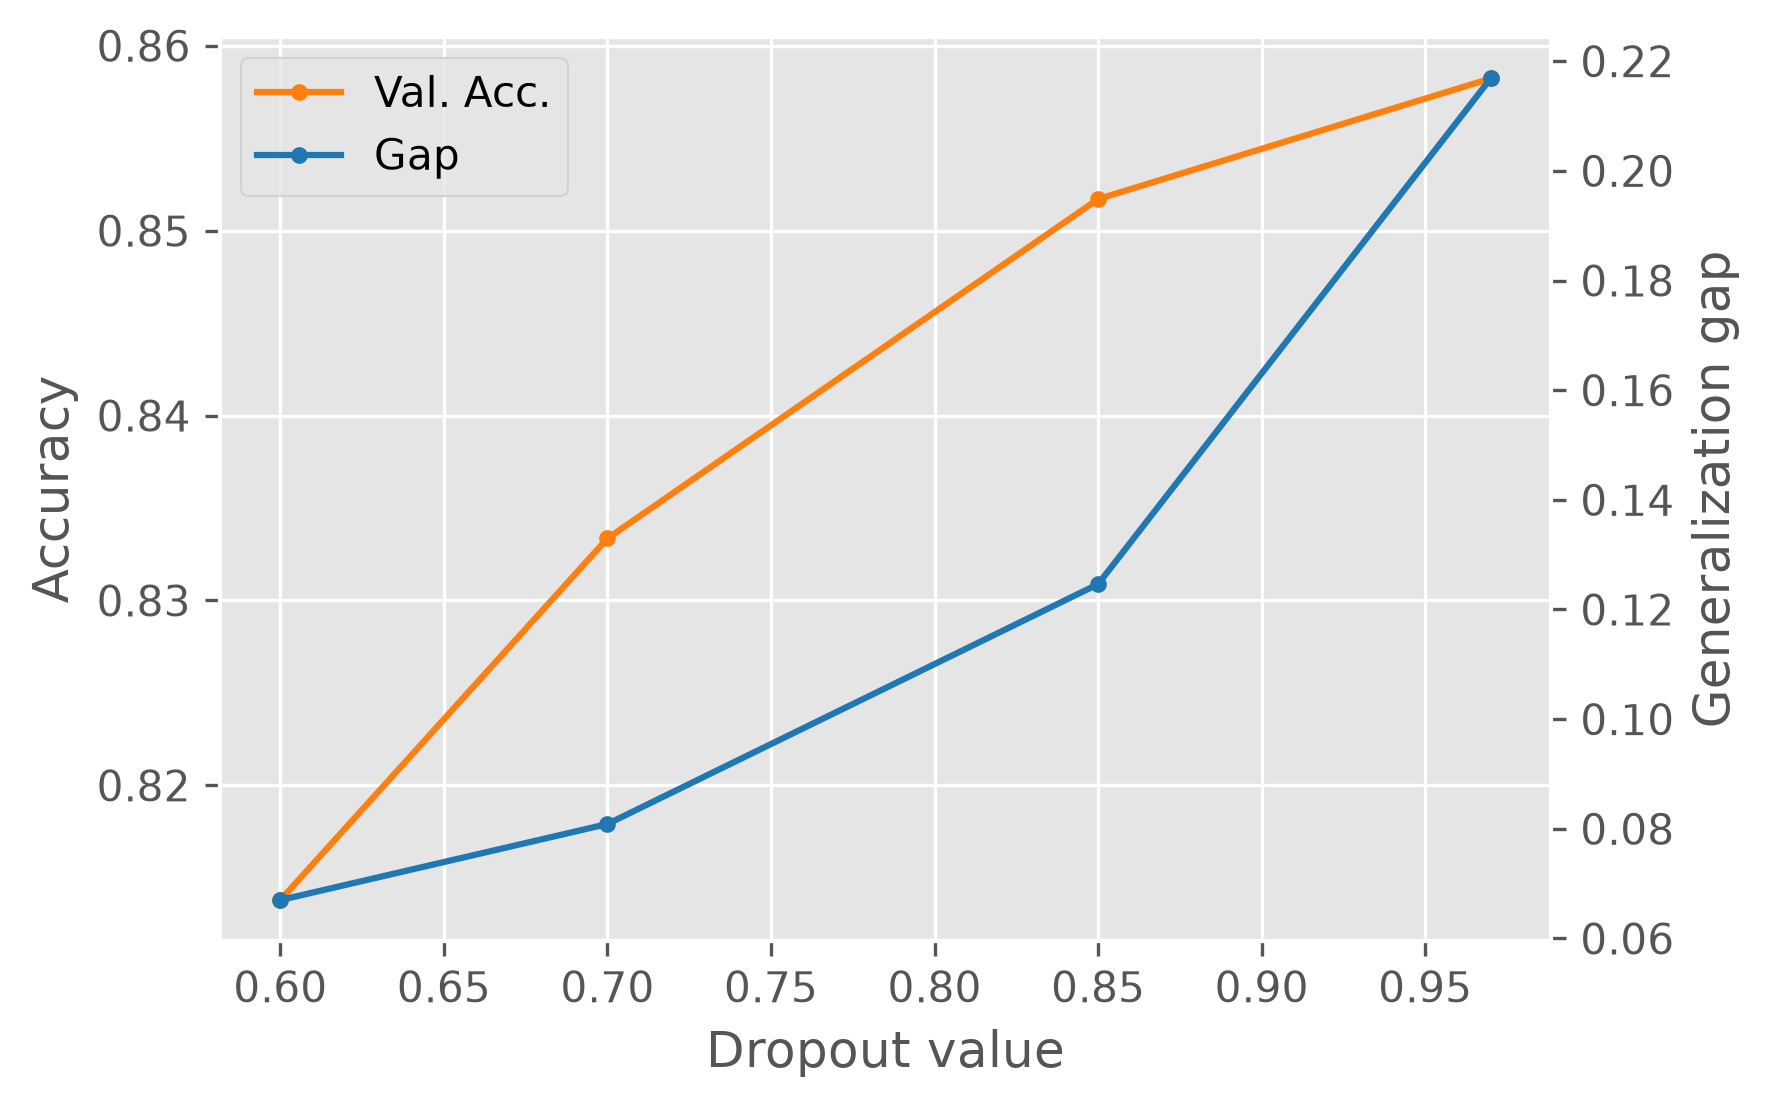
\includegraphics[width=\linewidth]{figures/dropout_accuracy.png}
        \caption{Validation accuracy and generalisation gap by inclusion probability.}
        \label{fig:dropoutrates}
    \end{subfigure} 
    \begin{subfigure}{.475\linewidth}
        \centering
        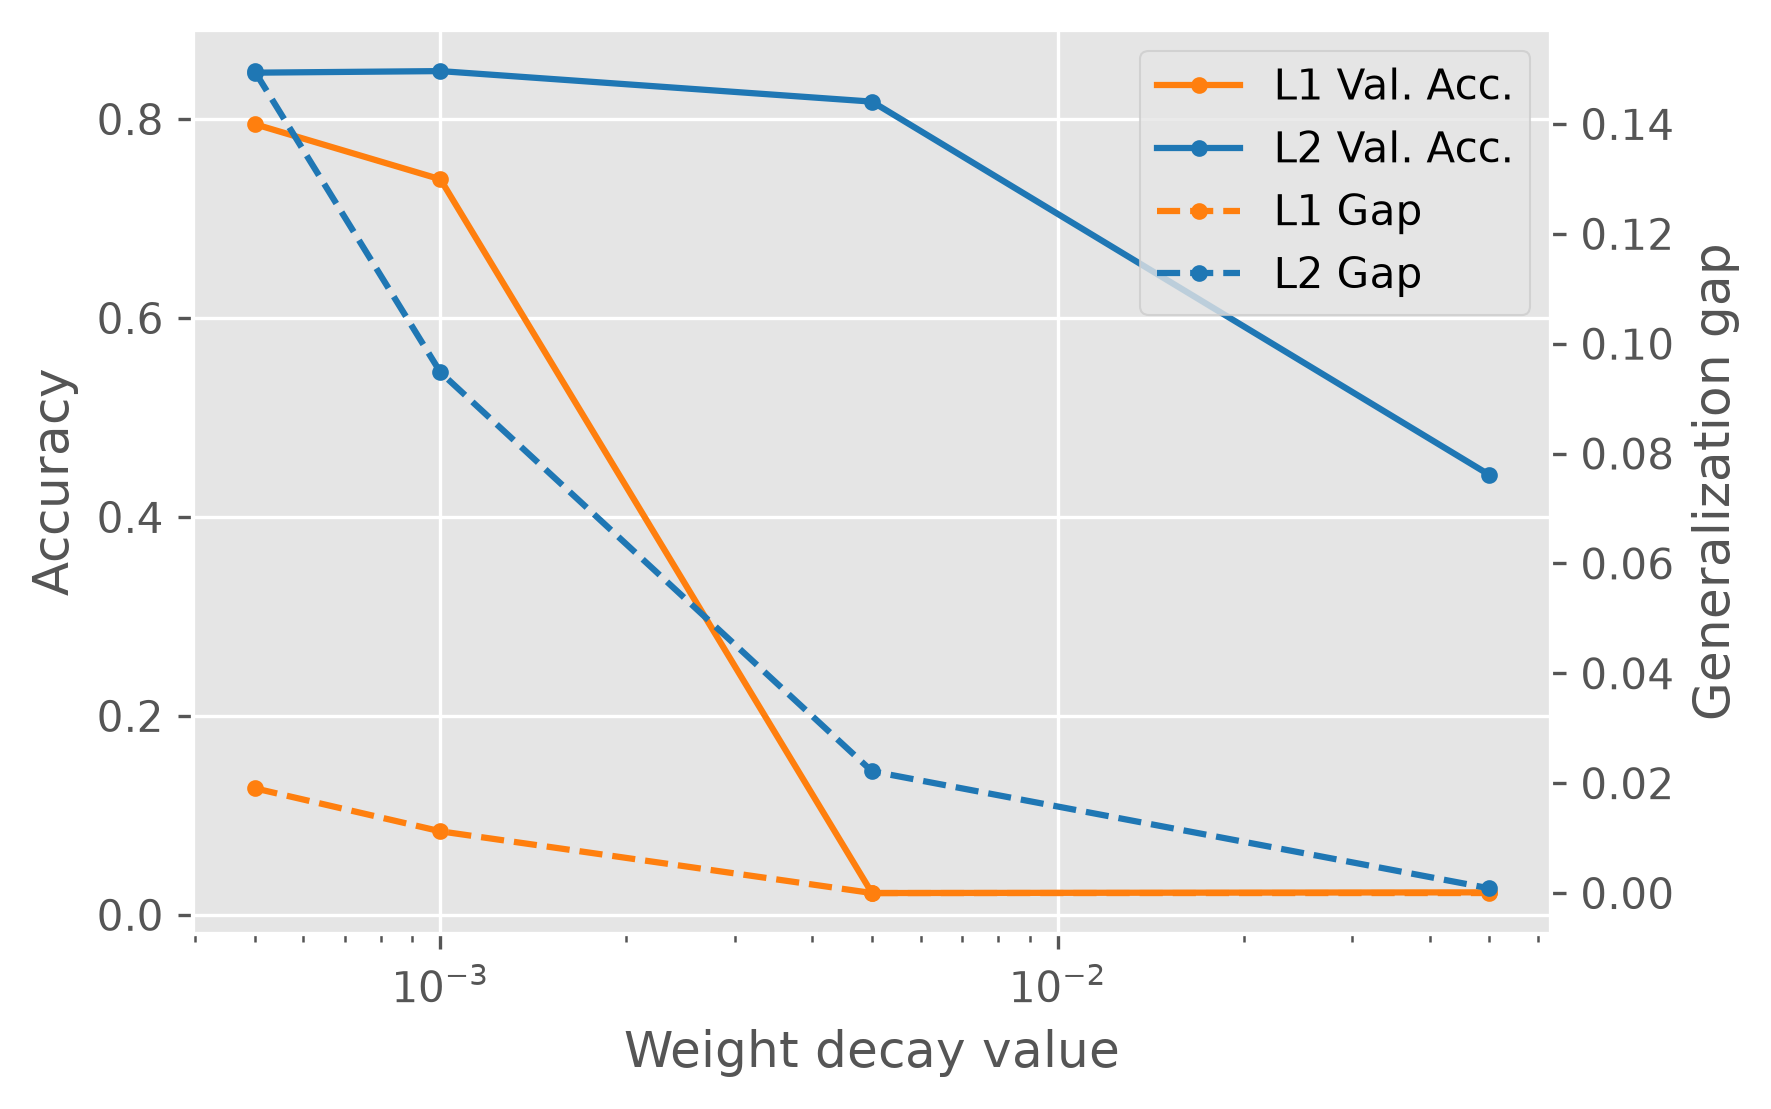
\includegraphics[width=\linewidth]{figures/regularization_accuracy.png}
        \caption{Validation accuracy and generalisation gap by penalty coefficient.}
        \label{fig:weightrates}
    \end{subfigure} 
    \caption{Epoch-100 validation accuracy and generalisation gap (validation minus training cross-entropy) against regularisation strength for dropout and L1/L2 regularisation.}
    \label{fig:hp_search}
\end{figure*}
}
}

%% Question Figure 5:
\newcommand{\questionFigureFive} {
\youranswer{Question Figure 5 - Add figures depicting the Validation Accuracy and Generalisation Gap (difference between validation and training error) for each of your 10 experiments depicted in Table 4.
}
}

%% Question Figure 6:
% \newcommand{\questionFigureSix} {
% \youranswer{Question Figure 6 - Add figures depicting the Training Accuracy, Error, and Gradient Flow Across Parameter Tensors for the one experiment run with the provided custom activation (produce these by running the "Problematic Training" cell in the Coursework\_1.ipynb notebook).
% }
% }

%% - - - - - - - - - - - - TABLES - - - - - - - - - - - - 

%% Question Table 1:
\newcommand{\questionTableOne} {
    \begin{table}[t]
        \centering
        \begin{tabular}{c|ccc}
        \toprule
        \# Hidden Units & Val. Acc. & Train Error & Val. Error \\
        \midrule
        32 & 78.9 & 0.556 & 0.694 \\
        64 & 81.1 & 0.339 & 0.665 \\
        128 & 80.7 & 0.159 & 0.964 \\
        \bottomrule
        \end{tabular}
        \caption{Epoch-100 validation accuracy (\%) and training/validation cross-entropy for one-hidden-layer ReLU networks on EMNIST.}
        \label{tab:width_exp}
    \end{table}
}

%% Question Table 2:
\newcommand{\questionTableTwo} {
    \begin{table}[t]
        \centering
        \begin{tabular}{c|ccc}
        \toprule
        \# Hidden Layers & Val. Acc. & Train Error & Val. Error \\
        \midrule
        1 & 80.7 & 0.159 & 0.964 \\
        2 & 81.5 & 0.092 & 1.599 \\
        3 & 81.8 & 0.119 & 1.739 \\
        \bottomrule
        \end{tabular}
        \caption{Epoch-100 validation accuracy (\%) and training/validation cross-entropy for ReLU networks with 128 units per hidden layer on EMNIST. Adam learning rate $10^{-3}$, batch size 100, seed 111020.}
        \label{tab:depth_exps}
    \end{table}
}

%% Question Table 3:
\newcommand{\questionTableThree} {
\youranswer{
Question Table 3 - Fill in Table 3 with the results from your experiments for the missing hyperparameter values for each of L1 regularisation, L2 regularisation, Dropout and label smoothing (use the values shown on the table). For Na\"ive Elastic Net, you need to implement the technique, choose an appropriate set of hyperparameter values, and report the results of one experiment in the table.
%
\begin{table*}[t]
    \centering
    \begin{tabular}{c|c|ccc}
    \toprule
        Model    &  Hyperparameter value(s) & Validation accuracy (\%) & Train Error & Validation Error \\
    \midrule
    \midrule
        Baseline &  -                    & 84.0 & 0.242 & 0.530 \\
    \midrule
        \multirow{4}*{Dropout}
                 & 0.6                   & 81.7 & 0.487 & 0.551 \\
                 & 0.7 & 83.34 & 0.405 & 0.486  \\
                 & 0.85 & 85.2 & 0.305 & 0.429 \\
                 & \textbf{0.97} & \textbf{85.6} & \textbf{0.229} & \textbf{0.447} \\
    \midrule
        \multirow{4}*{L1 penalty}
                 & \emph{5e-4} & \emph{79.6} & \emph{0.643} & \emph{0.663} \\
                 & 1e-3 & 73.94 & 0.873 & 0.885 \\
                 & 5e-3 & 2.19 & 3.850 & 3.850 \\
                 & 5e-2 & 2.13 & 3.850 & 3.850 \\
    \midrule
        \multirow{4}*{L2 penalty}  
                 & 5e-4 & 84.6 & 0.312 & 0.460 \\
                 & \emph{1e-3} & \emph{84.82} & \emph{0.361} & \emph{0.455} \\
                 & 5e-3 & 81.7 & 0.579 & 0.601 \\
                 & 5e-2 & 44.2 & 2.117 & 2.118 \\
    \midrule
        Label smoothing & 0.1 & 85.17 & 0.398 & 0.554 \\
    \midrule
        Na\"ive Elastic Net & 0.00005, 0.00005 & 84.72 & 0.329 & 0.457 \\
    \bottomrule
    \end{tabular}
    \caption{Results of the individual-method experiments.
Report epoch-100 results, matching the supplied entries,
with random seed 111020. Errors are ordinary cross-entropy
against the original, unsmoothed labels and exclude all
weight penalties. \emph{Italics} indicate the best configuration
for each method (dropout, L1 regularisation, L2 regularisation,
label smoothing and na\"ive elastic net), and \textbf{bold}
indicates the best configuration in this table. Rank
configurations by validation accuracy, using validation
cross-entropy to break ties.}
    \label{tab:hp_search}
\end{table*}
}
}


%% Question Table 4:
\newcommand{\questionTableFour} {
\youranswer{
Question Table 4 - Add a table with the results from your 10 experiments (by which we mean: 10 training runs, NOT 10 sets of experiments) varying different hyper-parameters and regularization combinations.
}
}

%% END of YOUR ANSWERS
